\documentclass[12pt]{article}
\usepackage[margin=1in]{geometry}
\usepackage{amsmath,amssymb}
\usepackage{booktabs}
\usepackage{enumitem}
\usepackage{siunitx}
\usepackage{hyperref}
\usepackage{graphicx} % for q3 graph pic
\hypersetup{colorlinks=true,linkcolor=black}
\sisetup{table-number-alignment=center,table-figures-integer=1,table-figures-decimal=3}

\title{ECON 695 Problem Set 6}
\author{Alejandro De La Torre}
\date{November 2, 2025}

\begin{document}
\maketitle

\noindent\textbf{Due: 11:59PM Central Time on Sunday 11/09/2025.}\\
\emph{Note: This problem set will be graded on a complete/incomplete basis. You’ll receive full credit for each question as long as you make a reasonable attempt. Use this problem set to study for Midterm 2.}

\bigskip

\section*{1. (2 points) Lecture 6 -- Head Start Impact Study}
In Lecture 6 we introduced the Head Start Impact Study, a nation-wide experiment in which Head Start (HS) seats are randomly assigned to families, and researchers use the experiment to assess the effects of HS on children’s school readiness and parental outcomes. 5,000 kids are randomly assigned to a treatment group (offered a HS seat) and a control group (no initial offer of HS seat). The table below comes from Bitler, Domina, and Hoynes (2015). Read the table and answer the following questions.

\begin{table}[h!]
  \centering
  \caption{Child care setting, by treatment or control status}
  \label{tab:hs_table2}
  \begin{tabular}{l S S S}
    \toprule
    & {Treatment Mean} & {Control Mean} & {Difference T--C} \\
    \midrule
    \emph{Head Start in HS Year} & & & \\
    Head Start (Administrative report) & 0.857 & 0.153 & 0.705\textsuperscript{***} \\
    \bottomrule
  \end{tabular}
\end{table}

\begin{enumerate}[label=\textbf{(\alph*)}, leftmargin=1.5em]
  \item Is the Head Start Impact Study a perfect randomized control trial (RCT)? Why or why not?\\[0.5em]
  
  \textbf{Solution.} \\
  The Head State Impact study is not a perfect RCT because we would likely not have complete compliance with regards to who takes the offered seat and who actually participates in the program. In a perfect PCT, treatment status is fully controlled where everyone assigned to treatment gets $D_i = 1$ and everyone assigned to control gets $D_i =0$ to get "full compliance", or everyone assigned to either control or treatment completely follow into their assigned groups. 
  
  In this context, this would mean forcing or expecting a family to take the head start seat upon recommendation, which would be problematic (CITI would come hunt you down). We observe from lecture 6 the first-stage regression,
    \[
    D_i=\hat\pi_0+\hat\pi_1 Z_i+\eta_i,
    \]
    with \(\hat\pi_0=E[D_i\mid Z_i=0]=0.153\) and \(\hat\pi_1=E[D_i\mid Z_i=1]-E[D_i\mid Z_i=0]=0.705\). These numbers mean some kids in the control group still attend preschool (\(\hat\pi_0>0\)) and some offered a seat do \emph{not} enroll (\(\hat\pi_1<1\)), that in fact there is cross-over between the treatment and control group in addition to incomplete take-up.

  \item Let $D_i=1$ if the kid attended preschool using a Head Start seat, and let $Z_i=1$ if the kid $i$ is assigned to the treatment group with initial offers of HS seats. If you estimate a first-stage regression of $D_i$ on a constant and $Z_i$, what are the estimates $\hat{\pi}_0$ and $\hat{\pi}_1$? Hint: use the numbers in the Table.
  \[
    D_i = \hat{\pi}_0 + \hat{\pi}_1 Z_i + \hat{\varepsilon}_i.
  \]

  % ANSWER HERE
  \textbf{Solution.} \\
  Upon estimating the first-stage regression of $D_i$ on a constant $Z_i$ as defined above, then the estimates $\hat{\pi}_0$ and $\hat{\pi}_1$ represent the following:
  \begin{itemize}
    \item The control mean represents the share of children in the same who attended the Head Start (HS) without being initially offered an HS seat which represents the coefficient: $\hat{\pi_0} = E[D_i | Z_i =0] = 0.153$
    \item The treatment mean represents the share of children who attended HS and were offered an HS seat, which is represented/can be estimated by: $E[D_i | Z_i = 1] = \hat{\pi_0} + \hat{\pi_1} = 0.857$
    \item The difference between the treatment and the control mean is exactly that, which is represented by $\hat{\pi_1}$ since $\hat{\pi}_1 = E[D_i | Z_i =1] - E[D_i | Z_i =0] = \left( \hat{\pi_1} + \hat{\pi_0} \right) - \hat{\pi_0} = (0.857) - 0.153 = 0.705$
  \end{itemize}
  In other words $\hat{\pi_1}$ represents the effect the offer on attendance in HS, or the compliance rate/share of compliers, whereas $\hat{\pi_0}$ represnts the "always-takers", or the share of students who attend the HS with-or-without an offer; the sum $\hat{\pi_1} + \hat{\pi_0}$ represents the students who attend HS with an offer.

  \item What does $\hat{\pi}_1$ represent? Hint: compliance.\\[0.5em]
  
  % ANSWER HERE
  \textbf{Solution.} \\
  I sort of answered it above, but $\hat{\pi_1}$ represents the share of compliers in the sample which in this context measures the effect of the offer of an HS seat has on HS attendance, which is in other words the compliance rate. This is calculated with the table of results as follows: $\hat{\pi}_1 = E[D_i | Z_i =1] - E[D_i | Z_i =0] = \left( \hat{\pi_1} + \hat{\pi_0} \right) - \hat{\pi_0} = (0.857) - 0.153 = 0.705$.

\end{enumerate}

\newpage

\section*{2. (2 points) Lecture 7 -- Local Average Treatment Effects (IV-LATE)}
Let $Y_i(d)$ denote a person $i$'s potential outcome when $D_i=d\in\{0,1\}$. Suppose there is an instrument $Z_i$ for $D_i$ that is randomly assigned $\big(D_i(0),D_i(1)\big)\ \perp\!\!\!\perp\ Z_i$ and satisfies the exclusion restriction, $Y_i(d,z)\equiv Y_i(d)$. We can use the IV--LATE framework to estimate the average treatment effects for some subpopulations (compliers under the monotonicity assumption). However, suppose there are some defiers with $D_i(0)=1$ and $D_i(1)=0$ that violate the monotonicity assumption. Consider the following first-stage regression and reduced-form regression:
\begin{align*}
  D_i &= \pi_0 + \pi_1 Z_i + \varepsilon_i,\\
  Y_i &= \delta_0 + \delta_1 Z_i + \nu_i.
\end{align*}

\begin{enumerate}[label=\textbf{(\alph*)}, leftmargin=1.5em]
  \item Derive expressions for the population estimates of the first-stage coefficient $\pi_1$. Show that if there are more compliers than defiers, then $\pi_1>0$.\\[0.5em]
  
  % ANSWER HERE
  \textbf{Solution.} \\
  We start from the first-stage regression equation:
    \[
    D_i = \pi_0 + \pi_1 Z_i + \varepsilon_i, \qquad E[\varepsilon_i \mid Z_i] = 0.
    \]
    The population OLS coefficient on $Z_i$ is given by the difference in conditional means:
    \[
    \pi_1 = E[D_i \mid Z_i = 1] - E[D_i \mid Z_i = 0].
    \]
    Using the random assignment of $Z_i$, we can write this as
    \[
    \pi_1 = E[D_i(1)] - E[D_i(0)] = E[D_i(1) - D_i(0)].
    \]

    We classify individuals by their treatment type based on $(D_i(0), D_i(1))$:
    \[
    \begin{cases}
    (0,0) & \text{Never-takers (NT)} \\
    (0,1) & \text{Compliers (C)} \\
    (1,0) & \text{Defiers (D)} \\
    (1,1) & \text{Always-takers (AT)}
    \end{cases}
    \]
    Let $\Pr(NT)$, $\Pr(C)$, $\Pr(D)$, and $\Pr(AT)$ denote the population shares of each group, with
    $\Pr(NT) + \Pr(C) + \Pr(D) + \Pr(AT) = 1$.

    Then we can compute the expected treatment rate for each instrument status:
    \[
    \begin{aligned}
    E[D_i \mid Z_i = 1] &= 0 \cdot \Pr(NT) + 1 \cdot \Pr(C) + 0 \cdot \Pr(D) + 1 \cdot \Pr(AT)
    = \Pr(C) + \Pr(AT), \\
    E[D_i \mid Z_i = 0] &= 0 \cdot \Pr(NT) + 0 \cdot \Pr(C) + 1 \cdot \Pr(D) + 1 \cdot \Pr(AT)
    = \Pr(D) + \Pr(AT).
    \end{aligned}
    \]

    Therefore, the population first-stage coefficient is:
    \[
    \pi_1 = E[D_i \mid Z_i = 1] - E[D_i \mid Z_i = 0] = \Pr(C) - \Pr(D),
    \]
    and the intercept is given by:
    \[
    \pi_0 = E[D_i \mid Z_i = 0] = \Pr(D) + \Pr(AT).
    \]

  Thus, the first-stage coefficient measures the difference in treatment take-up between the treatment and control groups. If there are more compliers than defiers ($\Pr(C) > \Pr(D)$), then $\pi_1 > 0$.

  \item Derive an expression for $\delta_1$ in the reduced form.\\[0.5em]
  
  % ANSWER HERE
  \textbf{Solution.} \\
  The reduced–form coefficient is the difference in mean outcomes across instrument status:
  \[
  \delta_1 \;=\; E[Y_i\mid Z_i=1]-E[Y_i\mid Z_i=0].
  \]
  Using the exclusion restriction $Y_i(d,z)\equiv Y_i(d)$ and random assignment, decompose each mean by principal strata $g\in\{\mathrm{NT},\mathrm{AT},\mathrm{Comp},\mathrm{Def}\}$:
  \begin{align*}
    E[Y_i\mid Z_i=1]
      &= E[Y_i(0)\mid \mathrm{NT}]\,\Pr(\mathrm{NT})
      \;+\;E[Y_i(1)\mid \mathrm{Comp}]\,\Pr(\mathrm{Comp})\\
      &\quad+\;E[Y_i(1)\mid \mathrm{AT}]\,\Pr(\mathrm{AT})
      \;+\;E[Y_i(0)\mid \mathrm{Def}]\,\Pr(\mathrm{Def}),\\[0.35em]
      E[Y_i\mid Z_i=0]
      &= E[Y_i(0)\mid \mathrm{NT}]\,\Pr(\mathrm{NT})
      \;+\;E[Y_i(0)\mid \mathrm{Comp}]\,\Pr(\mathrm{Comp})\\
      &\quad+\;E[Y_i(1)\mid \mathrm{AT}]\,\Pr(\mathrm{AT})
      \;+\;E[Y_i(1)\mid \mathrm{Def}]\,\Pr(\mathrm{Def}).
  \end{align*}
  Subtracting, terms for NT and AT cancel, yielding
  \[
  \delta_1
  = \big\{E[Y_i(1)-Y_i(0)\mid \mathrm{Comp}]\big\}\,\Pr(\mathrm{Comp})
  \;+\;\big\{E[Y_i(0)-Y_i(1)\mid \mathrm{Def}]\big\}\,\Pr(\mathrm{Def}).
  \]
  Equivalently,
  \[
  \delta_1
  = E[Y_i(1)-Y_i(0)\mid \mathrm{Comp}]\,\Pr(\mathrm{Comp})
  \;-\;E[Y_i(1)-Y_i(0)\mid \mathrm{Def}]\,\Pr(\mathrm{Def}).
  \]

  \emph{Link to the in-class result.} In lecture (with monotonicity), there are no defiers, so $\Pr(\mathrm{Def})=0$ and the second term drops. Hence
  \[
  \delta_1^{\text{(mono)}} 
  = E[Y_i(1)-Y_i(0)\mid \mathrm{Comp}]\,\Pr(\mathrm{Comp}),
  \]
  which is exactly the formula shown on the slide. Here, without monotonicity, the reduced form is the complier effect weighted by $\Pr(\mathrm{Comp})$ \emph{minus} the defier effect weighted by $\Pr(\mathrm{Def})$.
  \item What is $\delta_1/\pi_1$ when $\mathbb{E}[\,Y_i(1)-Y_i(0)\mid\text{Complier}\,]=\mathbb{E}[\,Y_i(1)-Y_i(0)\mid\text{Defier}\,]$?\\[0.5em]
  
  % ANSWER HERE
  \textbf{Solution.} \\
  From part (b), the reduced–form effect and first–stage are
    \[
    \delta_1
    = \big\{ E[Y_i(1)-Y_i(0)\mid \text{Comp}] \big\}\Pr(\text{Comp})
    \;-\; \big\{ E[Y_i(1)-Y_i(0)\mid \text{Def}] \big\}\Pr(\text{Def}),
    \]
    \[
    \pi_1 \;=\; \Pr(\text{Comp}) - \Pr(\text{Def}).
    \]
  Now impose the condition in the question that the complier and defier gains are equal:
    \[
    E[Y_i(1)-Y_i(0)\mid \text{Comp}] \;=\; E[Y_i(1)-Y_i(0)\mid \text{Def}] \;\equiv\; \tau .
    \]
  Substituting into the reduced form,
    \[
    \delta_1 \;=\; \tau\,\Pr(\text{Comp}) \;-\; \tau\,\Pr(\text{Def})
    \;=\; \tau\,\big\{\Pr(\text{Comp})-\Pr(\text{Def})\big\}
    \;=\; \tau\,\pi_1 .
    \]
  Therefore, provided $\pi_1 \neq 0$ (i.e., the share of compliers differs from the share of defiers),
    \[
    \frac{\delta_1}{\pi_1} \;=\; \tau
    \;=\; E[Y_i(1)-Y_i(0)\mid \text{Comp}]
    \;=\; E[Y_i(1)-Y_i(0)\mid \text{Def}] .
    \]
  Intuitively, when compliers and defiers have the same treatment effect, the reduced form just scales the common effect by the net fraction moved by the instrument, so the IV ratio recovers that common effect.

\end{enumerate}

\newpage

\section*{3. (2 points) Lecture 7 -- Characteristics of Compliers}
In Lecture 7 we presented a study on the health impacts of cesarean section (\emph{c}-section). The authors use whether a mother lives closer to a high (H) \emph{c}-section hospital as an instrument for delivery at a H rather than low (L) \emph{c}-section hospital. Hospital compliers refer to mothers who would choose to deliver at a H hospital if they live closer to a H hospital, but would have chosen a L hospital if they live closer to a L hospital instead. The figure below shows $\mathbb{E}[Y_{it}(0)\mid\text{Compliers}]$ and $\mathbb{E}[Y_{it}(1)\mid\text{Compliers}]$ at different days since birth.

\begin{figure}[h!]
  \centering
  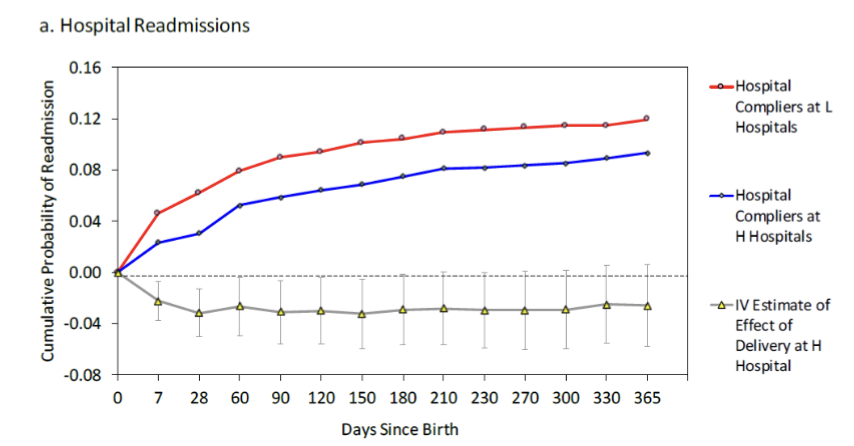
\includegraphics[width=0.85\textwidth]{../input/images/q3_hospital_admissions.png}
    \caption{Hospital Readmissions: $\mathbb{E}[Y_{it}(0)\mid\text{Compliers}]$ and $\mathbb{E}[Y_{it}(1)\mid\text{Compliers}]$}
\end{figure}

\begin{enumerate}[label=\textbf{(\alph*)}, leftmargin=1.5em]
  \item What is the first stage model? Does it vary by the days since birth (indexed by $t$ on the x-axis)?\\[0.5em]
  
  % ANSWER HERE
  \textbf{Solution.} \\
  Let $D_i$ denote the treatment “delivered at a high-$c$-section hospital (H)” and let $Z_i$ be the instrument indicating that the mother lives closer to an H than to an L hospital
  (relative distance). The outcome is indexed by days since birth $t$, so $Y_{it}$ is the (cumulative)
  probability of readmission by day $t$.

  \medskip
  \emph{First stage (take-up of $D_i$).}
  The population first-stage regression is
  \[
  D_i \;=\; \pi_0 \;+\; \pi_1 Z_i \;+\; \varepsilon_i,
  \]
  (optionally with covariates $X_i$: $D_i=\pi_0+\pi_1 Z_i+\pi_X'X_i+\varepsilon_i$).
  By random assignment and the exclusion restriction, the first-stage coefficient is
  \[
  \pi_1 \;=\; E[D_i\mid Z_i=1]-E[D_i\mid Z_i=0]
  \;=\; \Pr(\text{H-compliers}),
  \]
  i.e., the fraction of mothers whose hospital choice switches to H when $Z_i$ moves from $0$ to $1$.

  \medskip
  \emph{Does the first stage vary with $t$?}
  No. $D_i$ (delivery at an H hospital) is decided at the birth and therefore does not depend on
  the horizon $t$. The first stage $\pi_1$ is a single, time-invariant parameter that captures how
  $Z_i$ shifts the \emph{treatment} at delivery. What varies with $t$ is the \emph{outcome} $Y_{it}$ and,
  consequently, the reduced-form effect at horizon $t$,
  \[
  \delta_1(t)\;=\;E[Y_{it}\mid Z_i=1]-E[Y_{it}\mid Z_i=0],
  \]
  and the IV/LATE at each horizon,
  \[
  \frac{\delta_1(t)}{\pi_1}
  \;=\; E\!\big[\,Y_{it}(1)-Y_{it}(0)\,\big|\,\text{H-compliers}\big],
  \]
  which is interpreted as the average effect of delivering at an H hospital on readmissions
  \emph{by day $t$} for the complier subpopulation.

  \medskip
  \emph{Intuition.}
  The instrument changes \emph{who} delivers at an H hospital (compliers), and that margin is the
  same regardless of $t$. As we look farther out on the $x$–axis (days since birth), we track how
  the readmission outcome accumulates for those same compliers. Hence $\pi_1$ is fixed across $t$,
  while $\delta_1(t)$ and $\delta_1(t)/\pi_1$ trace out the time path of the complier effect.

  \item Set up a reduced-form regression of some ``goofy'' outcome on the proposed instrument that allows you to estimate $\mathbb{E}[Y_{it}(1)\mid\text{Compliers}]$ at a given $t$ (days since birth). Show what you can estimate in the reduced form, and how you can use it in combination with the first-stage regression to estimate $\mathbb{E}[Y_{it}(1)\mid\text{Compliers}]$.\\[0.5em]
  % ANSWER HERE
  \textbf{Solution.} \\

  At each horizon $t$ (days since birth), define the goofy outcome
  \[
  Y_{it}(1)\,D_i \quad\text{where}\quad
  Y_{it}(1)D_i =
  \begin{cases}
  Y_{it}, & D_i=1,\\
  0, & D_i=0.
  \end{cases}
  \]
  Consider the reduced-form regression of this goofy outcome on the instrument $Z_i$:
  \[
  Y_{it}(1)D_i \;=\; \delta_0(t) \;+\; \delta_1(t)\,Z_i \;+\; \nu_{it}.
  \]
  By definition of the reduced form,
  \[
  \delta_1(t)\;=\; E\!\left[Y_{it}(1)D_i \mid Z_i=1\right]
  \;-\; E\!\left[Y_{it}(1)D_i \mid Z_i=0\right].
  \]

  Use the exclusion restriction $Y_i(d,z)=Y_i(d)$ and random assignment $(D_i(0),D_i(1))\!\perp\! Z_i$ to decompose each mean by principal stratum $g\in\{\text{NT},\text{AT},\text{Comp},\text{Def}\}$:
  \[
  \begin{aligned}
  E\!\left[Y_{it}(1)D_i \mid Z_i=1\right]
  &= \sum_{g} E\!\left[Y_{it}(1)D_i(1)\mid g\right]\Pr(g)
  = E[Y_{it}(1)\mid \text{AT}]\,\Pr(\text{AT}) \\
  &\quad + E[Y_{it}(1)\mid \text{Comp}]\,\Pr(\text{Comp}), \\[4pt]
  E\!\left[Y_{it}(1)D_i \mid Z_i=0\right]
  &= \sum_{g} E\!\left[Y_{it}(1)D_i(0)\mid g\right]\Pr(g)
  = E[Y_{it}(1)\mid \text{AT}]\,\Pr(\text{AT}) \\
  &\quad + E[Y_{it}(1)\mid \text{Def}]\,\Pr(\text{Def}),
  \end{aligned}
  \]
  since $D_i(1)=1$ for AT and Compliers, and $D_i(0)=1$ for AT and Defiers.

  Therefore,
  \[
  \delta_1(t)
  = E[Y_{it}(1)\mid \text{Comp}]\,\Pr(\text{Comp})
  \;-\; E[Y_{it}(1)\mid \text{Def}]\,\Pr(\text{Def}).
  \]

  \emph{Link to the in-class (monotonicity) result.} In lecture the monotonicity assumption rules out defiers, $\Pr(\text{Def})=0$, so the second term vanishes and we get the simple formula
  \[
  \delta_1^{\text{(mono)}}(t)
  = E[Y_{it}(1)\mid \text{Comp}]\,\Pr(\text{Comp}).
  \]
  Combining with the first stage (from part (a)), $\pi_1=\Pr(\text{Comp})$, yields
  \[
  \frac{\delta_1^{\text{(mono)}}(t)}{\pi_1}
  = E[Y_{it}(1)\mid \text{Comp}],
  \]
  which is exactly what we want at horizon $t$.

  \noindent\textit{Note.} The first stage $\pi_1=\Pr(\text{Comp})-\Pr(\text{Def})$ is time-invariant, while the reduced form $\delta_1(t)$ varies with $t$ because $Y_{it}$ accumulates readmissions over days since birth. Without monotonicity, $\delta_1(t)$ identifies a weighted difference between complier and defier means and cannot by itself recover $E[Y_{it}(1)\mid\text{Comp}]$ unless $\Pr(\text{Def})=0$ or further assumptions are imposed.

  \item Repeat (b) for $\mathbb{E}[Y_{it}(0)\mid\text{Compliers}]$. Can you observe $\{Y_{it}(0)\}$ among compliers in the data?\\[0.5em]
  
  % ANSWER HERE
  \textbf{Solution.} \\

  At each horizon $t$, define the “goofy’’ outcome that reveals potential outcome under no treatment only when the unit is untreated:
    \[
    Y_{it}(0)\,(1-D_i)
    \qquad\text{where}\qquad
    (1-D_i)=
    \begin{cases}
    1, & D_i=0,\\
    0, & D_i=1.
    \end{cases}
    \]
    Run the reduced form on the instrument $Z_i$:
    \[
    Y_{it}(0)(1-D_i)\;=\;\tilde\delta_0(t)\;+\;\tilde\delta_1(t)\,Z_i\;+\;\nu_{it},
    \]
    so by definition
    \[
    \tilde\delta_1(t)\;=\;E\!\left[Y_{it}(0)(1-D_i)\mid Z_i=1\right]\;-\;E\!\left[Y_{it}(0)(1-D_i)\mid Z_i=0\right].
    \]

    Using the exclusion restriction $Y_i(d,z)=Y_i(d)$ and random assignment $(D_i(0),D_i(1))\!\perp\! Z_i$, decompose each mean by principal stratum $g\in\{\text{NT},\text{AT},\text{Comp},\text{Def}\}$:
    \[
    \begin{aligned}
    E\!\left[Y_{it}(0)(1-D_i)\mid Z_i=1\right]
    &=\sum_g E\!\left[Y_{it}(0)(1-D_i(1))\mid g\right]\Pr(g)\\
    &=E[Y_{it}(0)\mid \text{NT}]\,\Pr(\text{NT})\;+\;E[Y_{it}(0)\mid \text{Def}]\,\Pr(\text{Def}),\\[0.5em]
    E\!\left[Y_{it}(0)(1-D_i)\mid Z_i=0\right]
    &=\sum_g E\!\left[Y_{it}(0)(1-D_i(0))\mid g\right]\Pr(g)\\
    &=E[Y_{it}(0)\mid \text{NT}]\,\Pr(\text{NT})\;+\;E[Y_{it}(0)\mid \text{Comp}]\,\Pr(\text{Comp}),
    \end{aligned}
    \]
    since $D_i(1)=0$ for NT and Defiers (and $=1$ for AT and Compliers), while $D_i(0)=0$ for NT and Compliers (and $=1$ for AT and Defiers).

    Subtracting,
    \[
    \boxed{\;\tilde\delta_1(t)\;=\;-\;E[Y_{it}(0)\mid \text{Comp}]\,\Pr(\text{Comp})
    \;+\;E[Y_{it}(0)\mid \text{Def}]\,\Pr(\text{Def})\; }.
    \]

    \textit{Monotonicity link.} 
    If there are no defiers (monotonicity), $\Pr(\text{Def})=0$ and the reduced form simplifies to
    \[
    \tilde\delta_1^{(\text{mono})}(t)\;=\;-\;E[Y_{it}(0)\mid \text{Comp}]\,\Pr(\text{Comp}).
    \]
    Combining with the first stage from part (a), $\pi_1=\Pr(\text{Comp})$, we obtain
    \[
    \frac{-\,\tilde\delta_1^{(\text{mono})}(t)}{\pi_1}\;=\;E[Y_{it}(0)\mid \text{Comp}],
    \]
    which is exactly the complier mean of $Y_{it}(0)$ at horizon $t$.

  \textit{Can we directly observe $\{Y_{it}(0)\}$ for compliers?} 
    We observe $Y_{it}(0)$ for units with $D_i=0$ in the data, but we do not know which of those units are \emph{compliers} (as opposed to never-takers). Hence we cannot condition on complier status directly. The goofy reduced form above, combined with the first stage, recovers $E[Y_{it}(0)\mid\text{Comp}]$ under monotonicity; without monotonicity it delivers a mixture that also involves defiers, as shown in the boxed formula.

\end{enumerate}

\newpage

\section*{4. (2 points) Lecture 8 -- Panel Data -- Twins Study}
Suppose you are given data from surveys at the Twins Festival. Each family has a pair of identical twins. Let $i$ index a family and $t=1,2$ denote the twin \#1 and \#2. The goal is to use this panel data at $(i,t)$ or family $\times$ twin level to estimate the returns to education. Consider the following regressions of log earnings $Y_{it}$ on education $S_{it}$ (and other controls):

\begin{align}
Y_{it} &= \beta_0^{FE} + \beta_1^{FE} S_{it} + \alpha_i + \epsilon_{it} \tag{1}\\
Y_{it} &= \beta_0^{CF} + \beta_1^{CF} S_{it} + \bar{S_i}\gamma + u_{it} \tag{2}\\
Y_{it} &= \delta_0^{CF} + \delta_1^{CF} S_{it} + \delta_2^{CF} S_{i(-t)} + v_{it} \tag{3}
\end{align}

\begin{itemize}
  \item Model (1) controls for family fixed effects (controlling for dummies of each family $i$).
  \item Model (2) represents the control function approach with a control of $\bar{S_i} = \frac{S_{i1}+S_{i2}}{2}$, the mean education of the twins in the same family.
  \item Model (3) is an alternative control function that controls for $S_{i(-t)}$, which is the education of the identical twin instead of $\bar{S_i}$. For example, for twin $t=1$ in family $i$, $S_{i(-t)}=S_{i2}$ — education of his/her identical twin in the family.
\end{itemize}

\begin{enumerate}[label=\textbf{(\alph*)}, leftmargin=1.5em]
  \item Can you interpret $\hat{\beta}_1^{FE}$ as a causal estimate of return to education? State the assumption you need on model (1) to be able to consider $\hat{\beta}_1^{FE}$ as a causal estimate.\\[0.5em]
  
  % ANSWER HERE
  \textbf{Solution.} \\
  Consider the panel (family~$\times$ twin) model
\[
Y_{it} \;=\; \beta^{FE}_0 \;+\; \beta^{FE}_1\, S_{it} \;+\; \alpha_i \;+\; \varepsilon_{it},
\qquad i=\text{family},\; t\in\{1,2\},
\]
where $Y_{it}$ is log earnings for twin $t$ in family $i$, $S_{it}$ is that twin’s schooling,
$\alpha_i$ is a \emph{family fixed effect} (time-/twin-invariant unobservables shared by the pair),
and $\varepsilon_{it}$ is the time-/twin-varying error.

Applying the within (fixed-effects) transformation,
\[
Y_{it}-\bar Y_i \;=\; \beta^{FE}_1\,(S_{it}-\bar S_i) \;+\; (\varepsilon_{it}-\bar\varepsilon_i),
\]
so $\hat\beta^{FE}_1$ is estimated from variation \emph{within} families (i.e., differences across the twins).

\smallskip
\emph{Causal interpretation.}
We can interpret $\hat\beta^{FE}_1$ as the causal return to education (the effect of one more year of schooling on log earnings) \emph{holding fixed} all family-level time-invariant factors (genes, home background, etc.) \emph{if} the following assumptions hold:

\begin{enumerate}\setlength{\itemsep}{0.25em}
\item \textbf{Strict exogeneity (within family):}
\[
E\!\left[\varepsilon_{it}\,\middle|\, S_{i1},S_{i2},\alpha_i\right] = 0 \quad\text{for } t=1,2.
\]
Equivalently, the \emph{within-family} regressor $(S_{it}-\bar S_i)$ is uncorrelated with the \emph{within-family} error $(\varepsilon_{it}-\bar\varepsilon_i)$. 
Intuition: after netting out the family effect $\alpha_i$, there are no twin-specific shocks to earnings that are still correlated with twin-specific schooling.
\item \textbf{Within-family variation:} $\operatorname{Var}(S_{it}-\bar S_i)>0$ (the twins differ in schooling so the parameter is identified).
\item \textbf{Correct model for the fixed component:} all time-invariant unobservables relevant for earnings are absorbed by $\alpha_i$ (so they are allowed to be correlated with schooling, but do not vary across twins within a family).
\end{enumerate}

Under these conditions, the within estimator identifies
\[
\beta^{FE}_1 \;=\; \arg\min_b\, E\!\left[\big\{(Y_{it}-\bar Y_i) - b\,(S_{it}-\bar S_i)\big\}^2\right],
\]
which equals the causal effect of schooling on log earnings for the twins sample. 
(Practically, this is numerically equivalent to OLS with family dummies.)

  \textit{For questions (b)--(c), assume the correct assumption in (a) holds.}\\[0.5em]

  \item Show the within estimator in (1) is equivalent to the estimator from the control function — $\hat{\beta}_1^{FE} = \hat{\beta}_1^{CF}$.\\[0.5em]
  
  % ANSWER HERE
  \textbf{Solution.} \\

  \item How does $\hat{\beta}_1^{CF}$ relate the coefficients in (3) — $\hat{\delta}_1^{CF}$ and $\hat{\delta}_2^{CF}$? Clearly state the assumptions you use.\\[0.5em]
  
  % ANSWER HERE
  \textbf{Solution.} \\
\end{enumerate}

\newpage

\newpage
\section*{5. (2 points) Lecture 9 -- Difference in Differences}
In this question we will use potential outcomes to interpret the difference-in-differences model. Consider the classic Card and Krueger (1994) minimum wage study. Let $i$ denote a restaurant that either be in NJ or in PA (but not both -- ignore chains like McDonalds that have locations in both states). $t=1$ denotes the period before NJ raised minimum wage, and $t=2$ denotes the period after the change. As before, define $NJ_i=1$ if restaurant $i$ is in NJ, and $Post_t=1$ if $t=2$ (after the minimum wage increase).

Define the treatment variable as $D_{it}=NJ_i \times Post_t$, which equals to $1$ if the restaurant $i$ is in NJ, and $t=2$. The outcome of interest is full-time employment $Y_{it}$, and we want to estimate the difference-in-differences regression:
\[
  Y_{it}=\beta_0+\beta_1 NJ_i+\beta_2 Post_t+\beta_3 D_{it}+\epsilon_{it}.
\]

We can write the outcome as realized $Y_{it}=Y_{it}(D_{it})$. That is, $Y_{it}(0)$ is the potential full-time employment when there is no change in minimum wage, and $Y_{it}(1)$ is the potential outcome when the minimum wage is increased.

\begin{enumerate}[label=\textbf{(\alph*)}, leftmargin=1.5em]
  \item Can you estimate $\mathbb{E}[\,Y_{i1}(0)\mid NJ\,]$ and $\mathbb{E}[\,Y_{i1}(0)\mid PA\,]$ in the data? Explain why or why not.\\[0.5em]
  
  % ANSWER HERE
  \textbf{Solution.} \\

  \item Can you estimate $\mathbb{E}[\,Y_{i2}(1)\mid NJ\,]$ and $\mathbb{E}[\,Y_{i2}(1)\mid PA\,]$ in the data? Explain why or why not.\\[0.5em]
  
  % ANSWER HERE
  \textbf{Solution.} \\

  \item Use potential outcomes $\{Y_{it}(0),Y_{it}(1)\}$ to express the parallel trend assumption. Under the parallel trend assumption, what does $\beta_3$ represent?\\[0.5em]
  
  % ANSWER HERE
  \textbf{Solution.} \\
  
  
\end{enumerate}

\end{document}